
\documentclass[paper=a4, fontsize=11pt]{scrartcl} % A4 paper and 11pt font size
\usepackage[T1]{fontenc} % Use 8-bit encoding that has 256 glyphs
\usepackage[english]{babel} 
\usepackage{amsmath,amsfonts,amsthm} 
\usepackage{graphicx}
\usepackage{caption}
\usepackage{float}
\usepackage{subcaption}
\usepackage{paralist}
\setlength\parindent{0pt} % Removes all indentation from paragraphs - comment this line for an assignment with lots of text


\title{	
\normalfont \normalsize 
\textsc{Practical exercise with ARTS, OSF SoSe15} \\ [25pt] % Your university, school and/or department name(s)
%\horrule{0.5pt} \\[0.4cm] % Thin top horizontal rule
\huge Exercise 2: Atmospheric Brightness Temperature Spectra \\ % The assignment title
}

\author{sample solution}
\date{\normalsize\today} 

\begin{document}

\maketitle

\section{atmospheric zenith opacity}

Use the ARTS control file ``rtcalc.arts'' and Matlab plotting script ``plot\_bt.m'' to calculate and display the spectrum of atmospheric zenith opacity in the microwave spectral range for a midlatitude-summer atmosphere. There are four spectral lines in the plot. 

\begin{figure}[h!]
\centering
 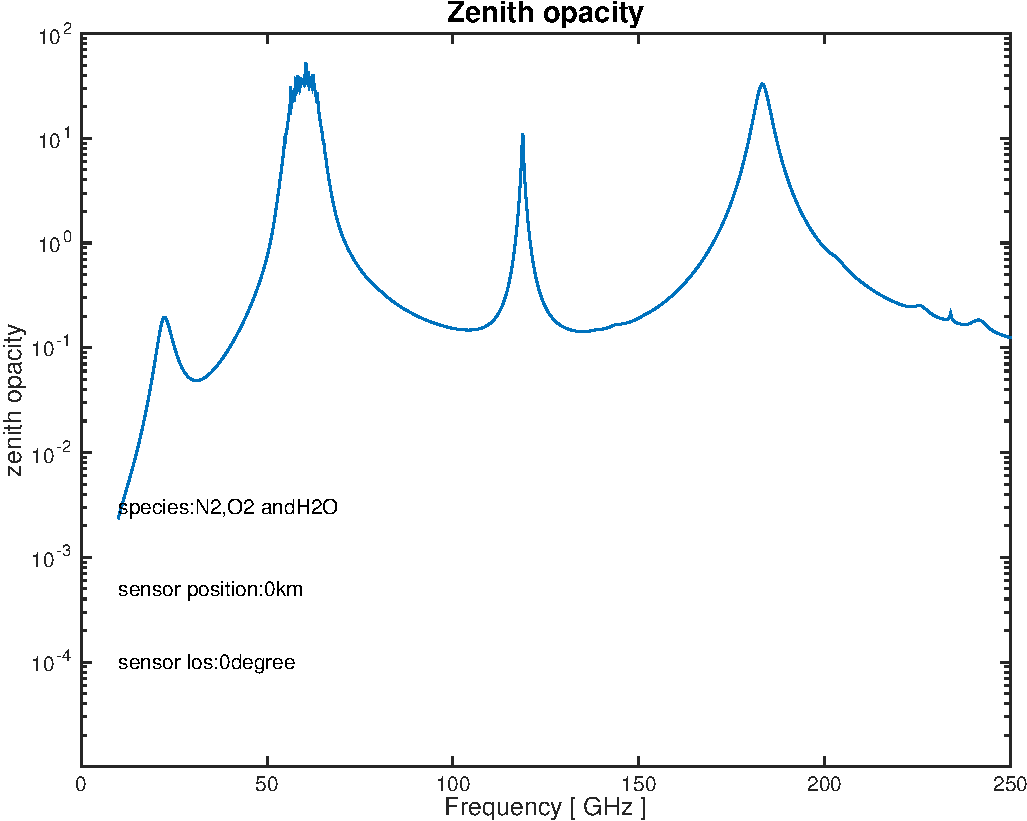
\includegraphics[width=0.8\textwidth]{plots/opacity_N2+O2+H2O_0km_0deg.pdf}
 \caption{zenith opacity}
\end{figure}

% figures abs cross sections
\begin{figure}[t!]
 \centering
 \begin{subfigure}[t]{0.45\textwidth}
 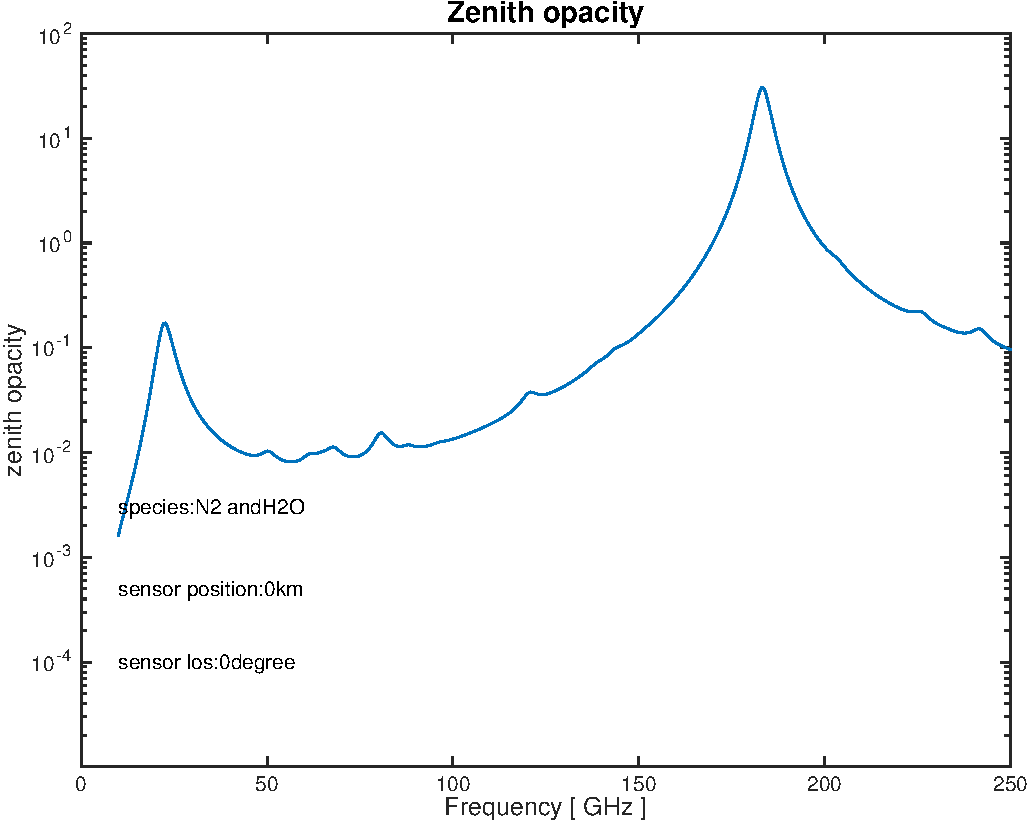
\includegraphics[width=\textwidth]{plots/opacity_N2+H2O_0km_0deg.pdf}
 \caption{$H_{2}O$ and $N_{2}$}
 \end{subfigure}
 \begin{subfigure}[t]{0.45\textwidth}
 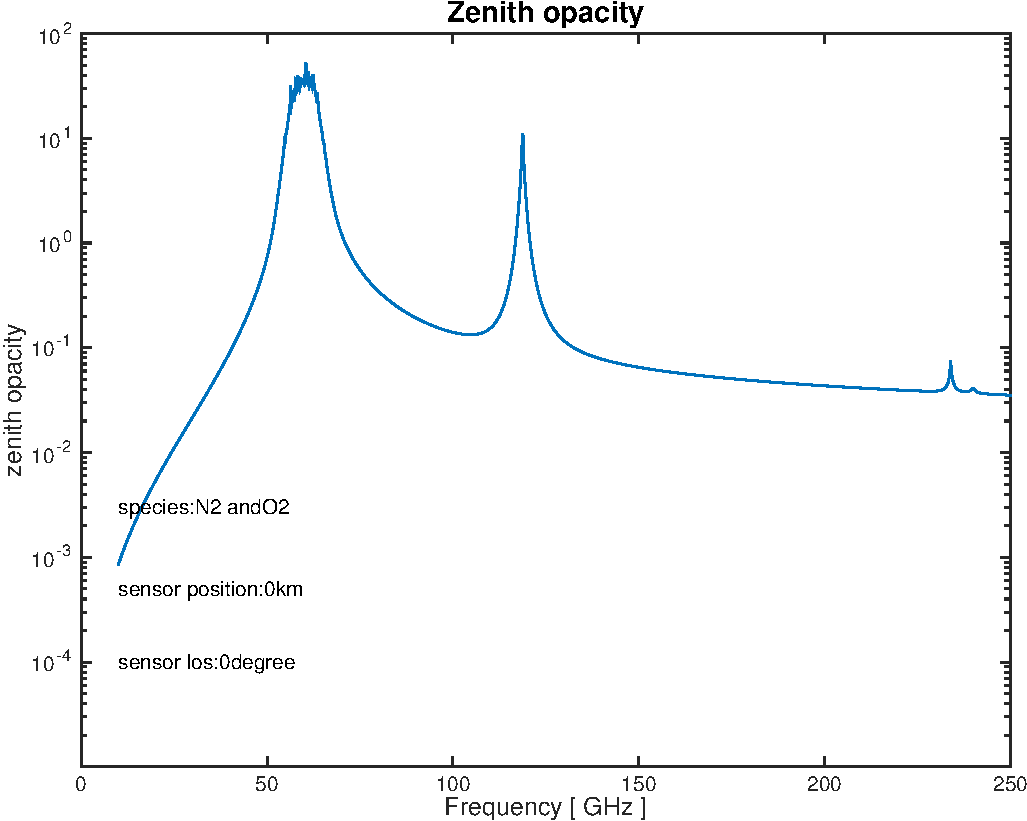
\includegraphics[width=\textwidth]{plots/opacity_N2+O2_0km_0deg.pdf}
 \caption{$O_{2}$ and $N_{2}$}
 \end{subfigure}
 \caption{zenith opacity seperately for $O_{2}$ and $H_{2}O$ molecules. }
 \label{figure:abs_molucules}
\end{figure}

\begin{itemize}
	\item To which species do these lines belong? (You can find this out by playing with the absorption species selection in the ARTS control file.)

	\item We speak of window regions where the zenith opacity is below 1. Where are they?

	\item Do you have any idea why $N_{2}O$ behaves like a diatomic molecule - and $O_{3}$ not?

\end{itemize}

%----------------------------------------------------------------------------------------
\ \\
\section{brightness temperature (bottom-up)}

Brightness temperature is a unit for intensity. It is the temperature that a blackbody should have to give the same intensity as measured. Mathematically, the transformation between intensity in SI units and intensity in brightness temperature is done with the Planck formula. Calculate and display the atmospheric brightness temperature spectrum for different hypothetical sensors:

\begin{compactenum}[a)]
\item A ground-based sensor looking in the zenith direction.
\item A sensor on an airplane (z = 10 km) looking in the zenith direction. 
\end{compactenum}

% figures abs cross sections
\begin{figure}[H]
 \centering
 \begin{subfigure}[h!]{0.46\textwidth}
 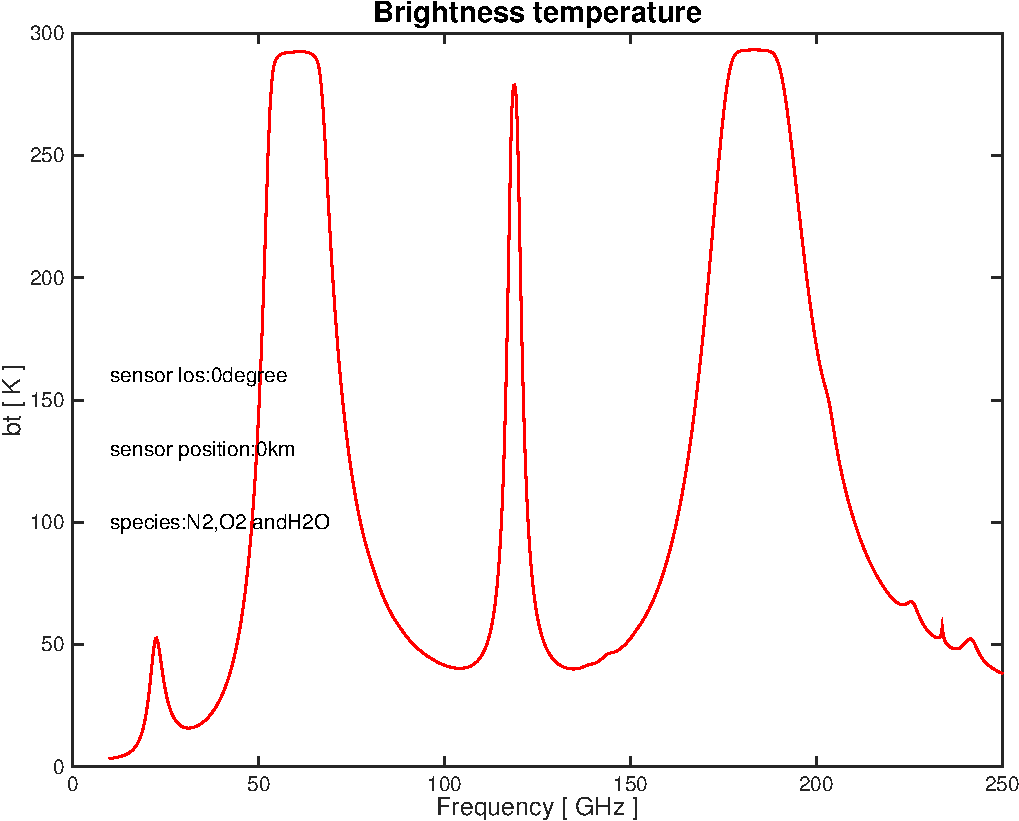
\includegraphics[width=\textwidth]{plots/bt_N2+O2+H2O_0km_0deg.pdf}
 \caption{ground}
 \end{subfigure}
 \begin{subfigure}[h!]{0.45\textwidth}
 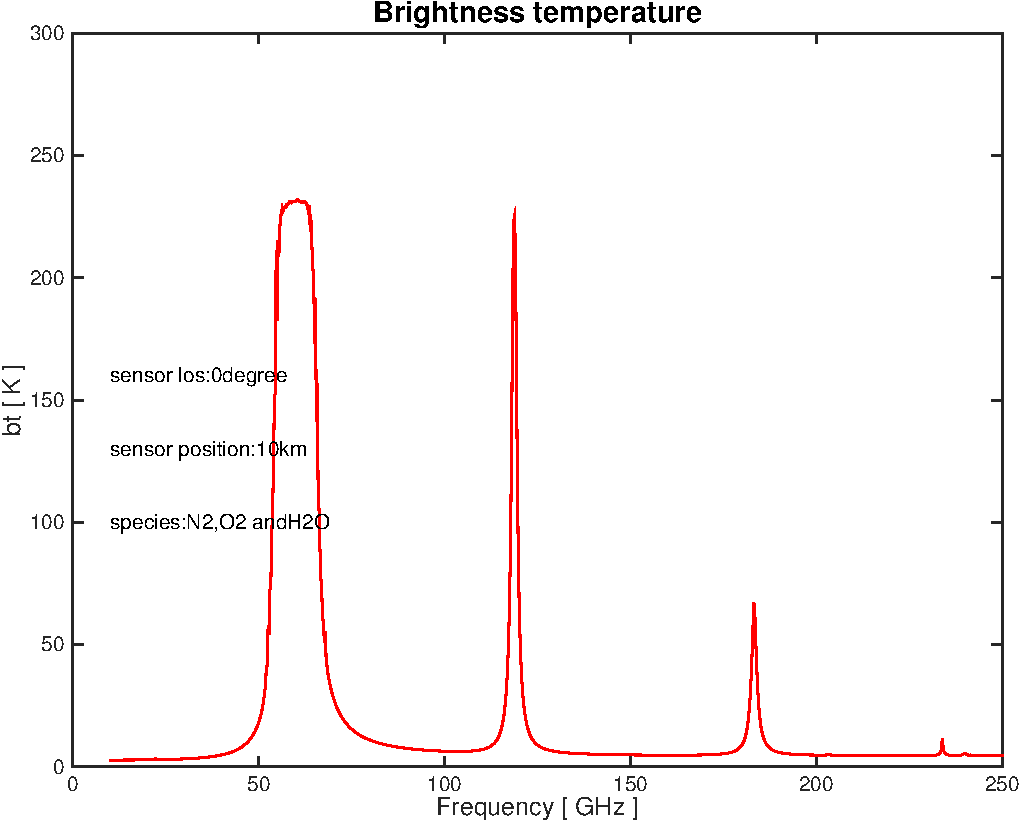
\includegraphics[width=\textwidth]{plots/bt_N2+O2+H2O_10km_0deg.pdf}
 \caption{10 km high}
 \end{subfigure}
 \caption{brightness temperatur for a sensor positioned at the ground and at 10 km height. }
 \label{figure:abs_pressure}
\end{figure}

\ \\
\textbf{Questions}
\begin{itemize}
	\item In Plot (a), why do the lines near 60 GHz and near 180 GHz appear flat on top?

	\item In Plot (b), why is the line at 180 GHz smaller than the line at 120 GHz, although its zenith opacity is higher?

	\item Describe the difference between plots (a) and (b). What happens to the lines, what happens to the background? Can you explain what you see?
\end{itemize}
%----------------------------------------------------------------------------------------
\ \\
\section{brightness temperature (top-down)}

Make the same calculation for a satellite sensor (z = 800 km) looking nadir (straight down). \ \\

\textbf{Questions}
\begin{itemize}
	\item Why is the line at 180 GHz 'upside-down', but the one at 20 GHz not?
	\item Explain the funny shape of the O2 line at 120 GHz.
\end{itemize}

\begin{figure}[H]
\centering
 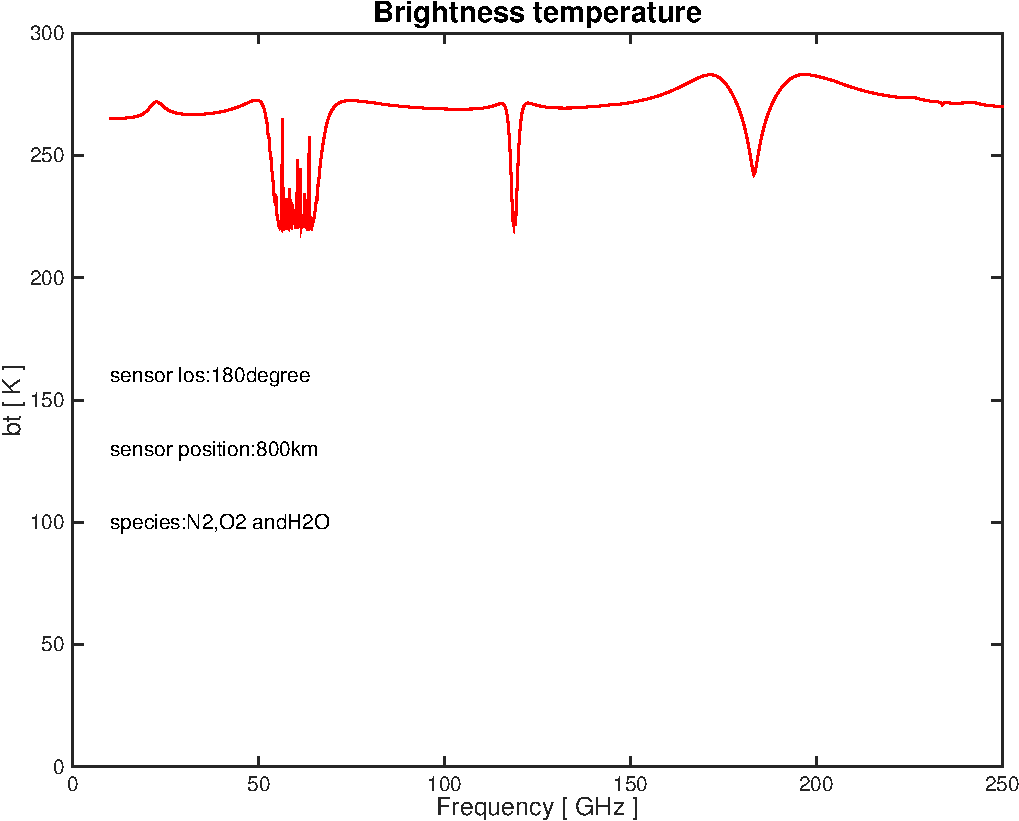
\includegraphics[width=0.6\textwidth]{plots/bt_N2+O2+H2O_800km_180deg.pdf}
 \caption{brightness temperature seen from a sensor looking down. }
\end{figure}





\end{document}
